
\section{Segmentations}

\begin{frame}
  \frametitle{Segmentation}
 
  \begin{block}{Definition}
A given range contains a finite set of segments verifying a valid property P. A segmentation is a subset of the whole set of segments, such that:
\begin{enumerate}
 \item each element of the range belongs to a segment of the subset
 \item no segment contains another segment of the subset 
\end{enumerate}
Due to (2), the segments of a segmentation can be ordered without ambiguity (according to the relative position of their first element for instance).
  \end{block}


  \begin{block}{Types}
SegmentComputerIterator
 \begin{itemize}
  \item dereference operator: return an instance of a segment computer.
  \item intersectPrevious(), intersectNext(): return 'true' if the current segment intersects, respectively, the previous and the next one (when they exist), 'false' otherwise.
 \end{itemize}
  \end{block}

  \begin{block}{Methods}
init method taking as input parameters: 
\begin{itemize}
 \item begin/end (circular)iterators of the range to be segmented
 \item an instance of segment computer
\end{itemize}
  \end{block}

\end{frame}


\begin{frame}[fragile]
  \frametitle{Greedy segmentation}

\begin{verbatim}

  //types definition
  typedef PointVector<2,int> Point;
  typedef std::vector<Point> Range;
  typedef Range::const_iterator ConstIterator;
  typedef ArithmeticalDSS<ConstIterator,int,8> SegmentComputer;
  typedef GreedySegmentation<SegmentComputer> Segmentation;


  Range curve;
  ... //create curve


  //Segmentation
  SegmentComputer recognitionAlgorithm;
  Segmentation theSegmentation(curve.begin(), curve.end(), recognitionAlgorithm);

                                 
  Segmentation::SegmentComputerIterator i = theSegmentation.begin();
  Segmentation::SegmentComputerIterator end = theSegmentation.end();
  for ( ; i != end; ++i) {
     SegmentComputer current(*i);
     trace.info() << current << std::endl;   //standard output
  }

\end{verbatim}


\end{frame}


\begin{frame}[fragile]
  \frametitle{Greedy segmentation}

\begin{verbatim}

...
  typedef Range::const_reverse_iterator ConstIterator;
...
  Segmentation theSegmentation(curve.rbegin(), curve.rend(), recognitionAlgorithm);
...

\end{verbatim}

 \begin{center}
   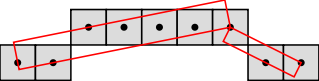
\includegraphics[width=0.45\textwidth]{left_right}
   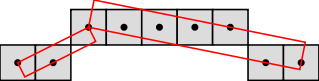
\includegraphics[width=0.45\textwidth]{right_left}
 \end{center}

\end{frame}

\begin{frame}[fragile]

  \frametitle{Saturated segmentation}

\begin{verbatim}

...
   typedef SaturatedSegmentation<SegmentComputer> Segmentation;
...

\end{verbatim}

 \begin{center}
   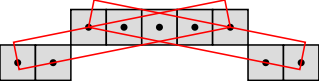
\includegraphics[width=0.45\textwidth]{maxseg}
 \end{center}

\end{frame}

\begin{frame}[fragile]
  \frametitle{Segmentation of subranges}

\begin{verbatim}

theSegmentation.setSubRange(beginIt, endIt);
theSegmentation.setMode("myMode");

\end{verbatim}

\begin{itemize}
 \item greedy
  \begin{itemize}
   \item "Truncate" (default)
   \item "Truncate+1"
   \item "DoNotTruncate"
  \end{itemize}
 \item saturated
  \begin{itemize}
   \item "First",
   \item "MostCentered" (default)
   \item "Last"
  \end{itemize}
\end{itemize}


\end{frame}
